\chapter{Power Measurements on Machine Learning Jobs}
\label{sec:power_measurements}

\todo{I feel like I should add a paragraph somewhere explaining what I want to measure}

\paragraph{Options for measuring power}

There are multiple options for measuring the power of a given computer. One way of classifying these options would be under them being either \emph{logical measurements} or \emph{physical measurements}.

Logical ones would create a model on some metrics and derive the used power. One example would be using Linux' \emph{perf} tool to read hardware performance counters. \todo{This needs some more here}

Advantages of choosing a logical approach would be that no external hardware is needed and that the overhead of the measurement would be low, as the hardware counters are being kept track of anyway. Disadvantages on the other hand would be that such a model would have to be created or chosen and would include some form of error as all models do.

Physical measurements follow another route; measurement devices would be put between the operating hardware and the power supply. The point where a power measuring device is inserted would dictate what could and could not be measured, a wall mounted measurement device could only measure all power going into a computer and not differentiate between individual programs.

Advantages of physical measurements are that they can give a more holistic measurement of a system as would be the case for a wall mounted measurement device. Portability is an issue however, unlike operating-system supported tools such as perf, a measurement device would need more effort to be used on another system (or be entirely not useable, for example when such devices are only rated for a certain power level).

Due to having a power-measurement tool on-site in our university and it allowing whole-system measurements directly, I chose to follow the physical measurement option. 

\paragraph{Measurement tool}

The concrete tool used is the \emph{Microchip MCP39F511N Power Monitor (henceforth called MCP)}, which can be inserted between the device to test and the wall mounted power supply. A picture of it can be found in figure \ref{fig:mcp}. The MCP can report the current power consumption in 10 mW steps, each 5ms.

\begin{figure}
    \missingfigure{A figure of the MCP, ask Sven about this}
    \caption[short]{The MCP}
    \label{fig:mcp}
\end{figure}

\todo{I could include an extra paragraph on why the MCP is cool, and what it does differently, perhaps. Was there anything cool? I vaguely remember some measurement devices having two capacitors to more accurately determine usage}

I then used \emph{pinpoint}, a tool for energy profiling that can use different inputs, among them being the MCP, to read out its data. 

\paragraph{The test environment}

The experiments were run on my personal computer, the components of that are listed via the \emph{hwlist} tool, with unnecessary columns and rows being redacted for brevity:

\begin{lstlisting}[language=bash, frame=single, numbers=none, caption={Hardware environment of the measurements}, basicstyle=\ttfamily]
   $ lshw -short -C processor -C memory -C display -C bus
Class          Description
==========================
bus            AB350 Gaming K4
memory         16GiB System Memory
processor      AMD Ryzen 5 1600X Six-Core Processor
display        GP104 [GeForce GTX 1070]
\end{lstlisting}

Information about the operating system is given via \emph{hostnamectl}, again some parts redacted:

\begin{lstlisting}[language=bash, frame=single, numbers=none, caption={Used operating system information}, basicstyle=\ttfamily]
    $ hostnamectl 
   Operating System: Ubuntu 24.04 LTS                
             Kernel: Linux 6.8.0-39-generic
\end{lstlisting}

\paragraph{Measured Program}

Machine learning (ML) was used as the main motivation for checkpoint \& resume scheduling in the related works\cite {wiesner_lets_2021} and thus was also chosen by me to be measured and modeled. 

The concrete model and framework is secondary for our measurement. In my case, a small model would be chosen in order to have fewer data points for processing as well as faster iterations on the measurement script. 

There is a vast amount of machine learning frameworks. For a high-level model, the feature set of the framework only needed to support checkpointing, resuming, and some basic form of logging. 
Glancing at the documentation of popular frameworks such as \emph{torch}, \emph{tensorflow}, and \emph{huggingface} shows that these features are commonly supported. 

With not much bias towards any framework, huggingface was chosen because my supervisor Felix supplied a sample "hello-world"-esque machine learning script for python \emph{roberta.py}\footnote{\url{https://github.com/Quacck/master-thesis/blob/main/power-measurements/roberta.py}}.

The huggingface trainer supports callbacks, I thus modified the code by adding timestamped logs. These "Events" would be output into another .csv File I could later use.\todo{Later use for WHAT?!}

\paragraph{Conducted Experiments}

A script \footnote{\url{https://github.com/Quacck/master-thesis/blob/main/power-measurements/measure_roberta.sh}} was created to execute each experiment. 

On a high-level view, the following experiments were conducted: 

\begin{enumerate}
    \item \label{experiment:full}Run the whole program start to finish
    \item \label{experiment:partial_checkpointed}Run it partially, checkpointing after some step, sleeping, resuming from that step
    \item \label{experiment:partial_checkpointed_aborted}Run it partially, checkpointing after some step but aborting before the next checkpoint. Then resume as above.
    \item \label{experiment:startup_only}Run only the startup phase up until the ML would start
    \item \label{experiment:baseline}Do nothing, measure the system at rest
\end{enumerate}

Experiment \ref{experiment:full} would give a baseline for what the job would look like without checkpoint \& resume. Number \ref{experiment:partial_checkpointed} and \ref{experiment:partial_checkpointed_aborted} would be used to determine the overhead of checkpointing the job. \ref{experiment:startup_only} would be used to validate the other ones. The last experiment is necessary to determine the baseline energy consumption of the environment.

To execute these experiments inside a repeatable bash script, additional command line parameters were added to the given python script. 
For example, there would be a boolean parameter \verb|--resume_from_checkpoint|, or an integer parameter \verb|--stop_after_epoch| would be used for experiment \ref{experiment:full} to \ref{experiment:partial_checkpointed}. 
The way of doing experiment \ref{experiment:startup_only} was to copy the script, and delete everything after the imports.

\paragraph{Creating repeatable measurements}

As this is being run on standard hardware on a standard operating system, all experiment are subject to noise. 
For example, \emph{Dynamic frequency and voltage scaling (DFVS)}, the OS technique of increasing CPU "speeds" according to work load would add power in an uncontrolled way. Also, background tasks may happen "randomly", increasing power usage. 

Thus, for the testing, any foreground apps would be closed. I also used the Linux tool \verb|cpupower|, as shown in snippet below, to set the CPU frequency to a set value:

\todo{Think about whether this is actually interesting, I guess keep it if I need more content}
\todo{What is the MAXFREQ of my Ryzen 5?}
\begin{lstlisting}[language=bash, frame=single, numbers=none, caption={Used operating system information}, basicstyle=\ttfamily]
    MINFREQ=$(cpupower frequency-info --hwlimits | sed -n '1d;p' \
        | awk '{print $1}')
    MAXFREQ=$(cpupower frequency-info --hwlimits | sed -n '1d;p' \
        | awk '{print $1}')
    
    cpupower frequency-set --min ${MAXFREQ} &>/dev/null
    cpupower frequency-set --max ${MAXFREQ} &>/dev/null

    # ... conduct experiments

    cpupower frequency-set --min ${MINFREQ} &>/dev/null
    cpupower frequency-set --max ${MAXFREQ} &>/dev/null
\end{lstlisting}
\label{listing:setting_cpu_frequency}

As machine learning makes use of available GPUs, the frequency should also be similarly set to a defined value. 
NVIDIA provides guide on how to do so\footnote{\url{https://developer.nvidia.com/blog/advanced-api-performance-setstablepowerstate}}.
Sadly, my used GPU, the NVIDIA GTX 1070, is not capable of fixing the frequency as of the time of conducting these experiments. 
While it is supposed to be possible according to\todo[inline]{SOURCE, Reconstruct this argument, perhaps there is still something in my PC history | grep}, but there seems to currently be drivers issue preventing this\todo{Find the forum post of people complaining}. 
Thus, the frequency of the GPU was not fixed. 
To reduce the effect of frequency scaling here, the time between experiments was increased generously so that any impact from such scaling would reoccur throughout each run and there would be reduced dependency between runs.

\todo{Further explain how the experiments were conducted}

\paragraph{Conducting each experiment}

Each experiment was re-run 10 times. Between each run, there would be a \verb|sleep| period of 10 seconds and one of two minutes in the partial executions. 
Additionally, \verb|pinpoint|'s feature of measuring before and after the actual program-to-test would be used. 
This leads to a period of 30 seconds being measured around the actual experiment. 
Plotting these additional time frames would give a quick visual indicator whether experiments are sufficiently isolated from each other, ergo when the power draw is at the baseline as the actual program starts.

As there is some data being downloaded and persisted during the execution of the ML, before each run, the data would be cleaned up.

\paragraph{Collected data}

For each experiment, a named and timestamped folder would be created in the \verb|/power-measurements| folder of my repository. Each folder would then hold a \verb|.csv| with pinpoint's timestamped power measurements. 
The added timestamped-logging would be saved into another \verb|.csv|. 
While figuring out how to conduct the experiments, I would then plot these measurements early and visually spot if there were any obvious errors or mistakes.

\paragraph{Determining the baseline power draw}

Beginning with the most exiting experiment, determining the baseline and testing the amount of the underlying environment. 
One sample run is shown in Figure \ref{fig:plot_baseline}.
The blue dots in figure represent each data point. The red line is a smoothed Gaussian trend line with $\sigma = 2$. 
Dark-green vertical lines are the logged or derived "events" for each run. In this case, nothing happens, so it is only the start and end of \verb|sleep 120|. 
Notice how the trace starts 30 seconds before the start and continues for another 30 seconds because of the aforementioned \verb|pinpoint| feature.
Going further, these additional measurements will be redacted for brevity, unless something worth mentioning happens outside the actual experiments.\todo{Check later if something interesting happens or if I should reword this.}

\begin{figure}
    \includegraphics[width=\linewidth]{power-measurements/measurements_sleep_0714004033/plot.pdf}
    \caption{Sample run of the baseline experiment}
    \label{fig:plot_baseline}
\end{figure}

Across all 10 runs, the average baseline power draw is calculated via the mean of all data points. This comes out as an average of 49.8 W with a standard deviation of 4.4 W.

The baseline power draw will be less interesting going further, but will put perspective on the power draws of the other experiments. The standard deviation should give a broad idea of how much noise is in the system environment.

\paragraph{The non-interrupted run}

For the non-interrupted machine learning run, a figure of a sample run is provided in \ref{fig:plot_full}. 
Figure \ref{fig:plot_full_stacked} shows the stacked trend lines of the 10 different runs.
For simplicity's sake, I refrained from doing more elaborate statistical analysis on the different runs as the visual check of them being very similar seemed enough. 
There was an option to discuss the measurement results after normalizing each measurement point to its phase, but that would not change the result.\todo{What?}

\begin{figure}
    \includegraphics[width=\linewidth]{power-measurements/measurements_roberta_full_0714010405/plot.pdf}
    \caption{Sample run of the full run experiment}
    \label{fig:plot_full}
\end{figure}

\begin{figure}
    \includegraphics[width=\linewidth]{power-measurements/stacked_plots/roberta_full_0714.pdf}
    \caption{Stacked trend lines of the power consumption for the full runs}
    \label{fig:plot_full_stacked}
    \todo[inline]{These are not yet accurate, the multiple evaluate phases are being grouped into one, which is wrong.}
\end{figure}

The main takeaways from these measurements are:

\begin{enumerate}
    \item There is a long (about 25\%) start-up phase, which is spent in starting python, loading libraries, and loading data to disc.
    \item There are periodical work-phases; a high-power training phase would be followed by low-power evaluation\todo{Uhm, where did my evaluation phase markers go?? They are mushed together as they share a label} phase and a low-power checkpointing.
    \item A higher variance in measurements occurs during the training phases in comparison to the others.
\end{enumerate}

This already shows, that improvements upon the constant-power model used in \cite{wiesner_lets_2021} are possible. 
For example, in this case the start-up phase has a much lower power-draw than the work-phase.

\paragraph{Results of the checkpoint and restore experiment}

Similarly to before, results will be discussed using the stacked plots \ref{fig:plot_partial_saved_stacked} and \ref{fig:plot_partial_saved_continue_stacked}; each individual run is plotted in the repository, however.

\begin{figure}
    \includegraphics[width=\linewidth]{power-measurements/stacked_plots/roberta_stop_after_saving.pdf}
    \caption{Power draws of the ML up until stopping after epoch 2}
    \label{fig:plot_partial_saved_stacked}
\end{figure}

\begin{figure}
    \includegraphics[width=\linewidth]{power-measurements/stacked_plots/roberta_continue_after_saving.pdf}
    \caption{Power draws after continuing from the second checkpoint}
    \label{fig:plot_partial_saved_continue_stacked}
\end{figure}

Here we can observe that

\begin{enumerate}
    \item The amount of work done is the same. 
    Similarly to the full-run experiment, the ML still takes the full 5 epochs and has the same work-phases
    \item There is no overhead from checkpointing itself, as the checkpoints are being created regardless of them being resumed from later.
    \item Resuming the jobs results in an added start-up phase. This phase is slightly shorter by a few seconds than the ones in the full runs, likely due to not needing to download the dataset again.
\end{enumerate}

Additional considerations are that the amount of epoch that are worked off before checkpointing and resuming may matter, but it will be assumed that this is not the case.\todo{I could just run this again with another epoch parameter}

\paragraph{Results from checkpoint and resume with abort}

Unlike the previous experiment, where work is stopped as soon as checkpoint is created, this time the program will be stopped just before a checkpoint is created (in this case just the second checkpoint would be saved). 
This should show the maximum created overhead from a checkpoint \& resume strategy. 

While this may sound artificial, it could happen in environments where the interaction between the scheduler and the job is not well orchestrated, for example in an environment where jobs are stopped "at random" like in a cloud spot instance.\todo{Improve the wording here}

Again, the results are visualized in figure \ref{fig:plot_partial_abort_stacked} and \ref{fig:plot_partial_abort_continue_stacked}. Attention should be paid to:

\begin{enumerate}
    \item The behavior of the repeated start-up phase is kept
    \item There is now a full additional training phase added to the overall work
\end{enumerate}

\begin{figure}
    \includegraphics[width=\linewidth]{power-measurements/stacked_plots/roberta_stop_without_saving.pdf}
    \caption{Power draws of the ML up until stopping after epoch 2}
    \label{fig:plot_partial_abort_stacked}
\end{figure}

\begin{figure}
    \includegraphics[width=\linewidth]{power-measurements/stacked_plots/roberta_continue_after_not_saving.pdf}
    \caption{Power draws after continuing from the second checkpoint}
    \label{fig:plot_partial_abort_continue_stacked}
\end{figure}

\paragraph{Calculating the energy costs of each run}

To support the argument that there is indeed an overhead from checkpointing \& resuming, I calculated the energy needed via integral of each experiment:

\begin{itemize}
    \item  unstopped costs 12.97 kJ on average with an std of 0.04
    \item  save+resume costs 13.94 kJ on average with an std of 0.1
    \item  save+abort+resume costs 15.72 kJ on average with an std of 0.07
\end{itemize}